\chapter{Conclusions}
\label{chap:discussion}
\newpage
\noindent
The aim of this thesis is the evaluation, development and application of robust methods to strengthen the raw material supply of a growing bio-economy sector. The success of bio-based companies depends, in part, on decisions that are made by foresters. Supporting forest management decisions is, therefore, beneficial, not only for the forest sector itself but also for wood processing companies. If forest enterprises and bio-economy companies are not able to contractually agree on continuous wood supply quantities, the success of a promising innovative bio-economy sector might be endangered \citep[p. 221, 223]{elchichakli_2016}. In a wood scarcity scenario, distribution decisions can have substantial consequences for wood processing companies, which depend on wood as a raw material. Rational and objective decisions of the wood distribution are therefore not only important for the forestry but also of the bio-economy sector. This reinforces the importance of DSS in the forest management decision process, as they can be used to structure the entire planning process of wood distribution into solvable sub-problems \citep[p. 1065-1067]{pretzsch_2008}. The benefits, disadvantages and results of the distinct statistical models developed here for decision support are discussed in the following.

\section{Findings of the thesis}
\label{sec:discussion:findings}
The introductory hypothesis, that matching demands of the rising bio-economy is actually problematic, was verified in chapter \ref{chap:hzb}. Scarcity of woody biomass and the high complexity of the entire wood supply chain are problems that forest enterprises and bio-economy companies have to cope with. A descriptive analysis of recent wood potential and wood usage reveals the significance of the research question and thus confirms the need for profound systems to help solve the anticipated raw wood distribution problem. After confirmation of the relevance of the introductory question in chapter \ref{chap:hzb}, the normative analysis in chapters \ref{chap:bm} to \ref{chap:opt} examine particular reasons why decision-makers may not be able to exploit the wood potential fully and how optimal potentials could be calculated.

\subsection{Analyzing status and development of raw wood availability in European beech-dominated central Germany}
\label{subsec:discussion:struct:hzb}
The available wood potential of all European beech wood assortments was almost completely exhausted in central Germany in the period between 2002 and 2012 (chapter \ref{chap:hzb}). Though the European beech wood potential is expected to rise due to ongoing forest development programs, competition on the wood market will probably rise. The only way for upcoming bio-economy companies to establish on the wood market is, thus, to compete with existing market participants. A detailed analysis of the wood market is, therefore, a prerequisite for the success of wood processing companies.

The added value of stem wood is higher than those of any other assortment \citep{nagel_2008}. The stem wood supply is currently entirely exhausted by long-established wood processing companies. It is therefore very difficult for novel companies to establish immediately on the stem wood market. Smaller-dimensioned, low-valued wood assortments make up about 60 \% of the available European Beech wood (chapter \ref{chap:hzb}). Although this low-valued wood is currently almost entirely used as well, availability is forecast to be better in the future. Approximately half of the wood potential of smaller dimension wood is directly used energetically. If a bio-economy company is able to compete with industrial wood and firewood prices, a solid base of renewable biomass from forests will then become available. This would be beneficial for the forest sector as well because the added value of sorting would increase \cite[p. 67]{mohring_1997}.

Two lessons should be learned from the predicted wood scarcity. First of all, the achievable sustainable wood potential should be estimated as accurately as possible in order to evaluate sources properly. Accurate estimations may uncover currently unused resources. Secondly, decisions on the distribution of the available wood potential must be made very carefully because the success of wood processing companies crucially depends on continuous wood supply quantities. Decisions on distribution of sparse resources can hence have serious consequences for forestry enterprises as well as for wood processing companies.

\subsection{Biomass functions and nutrient contents of European beech, oak, sycamore maple and ash and their meaning for the biomass supply chain}
\label{subsec:discussion:struct:bm}
The findings from chapter \ref{chap:bm} can improve harvest efficiency by making possible the gathering of the complete biomass potential of mixed deciduous forest sites. A comparison of several existing models revealed that the introduced models can significantly improve the estimation accuracy of biomass and nutrient contents in mixed deciduous tree species sites. This might help in identifying, and harvesting, formerly unused potential. The essay is particular relevant for the bio-based sector as innovative production methods often require biomass from deciduous tree species \citep[p. 1]{auer_2016} and the frequency of mixed deciduous stands is increasing steadily \citep{ti_2014}. The models enhance the accuracy of tree-specific biomass estimations. They can thus strengthen the planning accuracy of entire biomass supply chains.

\subsection{Modelling the economically viable wood in the crown of European beech trees}
\label{subsec:discussion:struct:beech_crowns}
The models from chapter \ref{chap:beech_crowns} are aimed at assessing the optimal wood volume in the crowns of European beech. They can thus be used to predict the full economically viable potential of smaller wood assortments. Allometric analysis revealed large wood potential in the crowns of deciduous trees. It is therefore essential to consider the predicted wood volume from the crown, a by-product of stem wood production. As the dimension of the wood assortments plays a minor role for many activities (subsection \ref{subsec:intro:struct:bm}), gathering further wood potential from deciduous crowns would seem to be of interest for bio-economy companies. The models also allow a precise prediction of harvestable wood volume prior to harvesting. They can therefore enhance the forecasting of volume flows in the biomass supply chain.

The model is able to calculate the maximal wood potential from an economic perspective only. It is therefore a purely normative-based model that predicts a rational, rather than a realistic, wood potential. Further economic or non-economic endogenous influences, such as fixed assortment lengths or maximum small-end diameters, cannot be considered in the model. It enables the calculation of the maximal tree-specific wood amount but it does not predict actual decisions.

\subsection{Case studies of the combined simulation-optimization approach}
\label{subsec:discussion:struct:opt:application}
\subsubsection{Motivation}
\label{subsubsec:discussion:struct:opt:application:introduction}
The following subsection provides supplemental information about the development and the interpretation of the two examples from chapter \ref{chap:opt}. Chapter \ref{chap:opt} introduces the statistical and technical foundations of the optimization module that builds the core element of the simulation-optimization model. The high demands of forest schedule optimization on the optimization method are illustrated and discussed in subsection \ref{subsec:intro:struct:opt} and section \ref{sec:opt:Introduction}. A Simulated-Annealing based optimizer, specifically developed for usage in an optimization-optimization software, is presented. The applicability of the \texttt{optimization} package for optimization of forest harvesting is briefly confirmed in two practical examples. In the following, the two examples from subsection \ref{subsec:opt:examples:forest} are described in more detail. The detailed descriptions of the examples facilitate the discussion and the findings with view to research question (Section \ref{sec:intro:aim}).

To explain its basic behavior and to confirm its practical applicability for forest enterprises, the si\-mu\-la\-tion-op\-ti\-mi\-za\-tion software was performed on two exemplary forest enterprises to optimize their harvesting intensity. The two example enterprises were generated to explain and discuss how the si\-mu\-la\-tion-op\-ti\-mi\-za\-tion software can be used to support decisions of the intermediate-term forest planning. The first exemplary enterprise was created to show the basic behavior of the si\-mu\-la\-tion-op\-ti\-mi\-za\-tion software. It is comprised of five forest stands that were specifically chosen for exemplary purposes. The second exemplary enterprise was composed such that it represents a typical forest enterprise of central Germany covering all relevant age classes of European beech. The second example explains the reasonability of the si\-mu\-la\-tion-op\-ti\-mi\-za\-tion approach for typical forest enterprises of the most important region for the supply of the wood-based bio-economy industry (Section \ref{sec:hzb:Einleitung}).

Three simulation scenarios were calculated for both forest enterprises. The forest developments and the wood potentials of both exemplary enterprises were firstly forecasted without any optimization using the TreeGrOSS growth and yield simulation packages without any optimization. The results were compared with the optimized treatment simulations in the framework of a sensitivity analysis. Accordingly, in the second scenario, the stand harvesting intensities were optimized using the combined simulation-optimization approach (Figure \ref{fig:Introduction:flowopt}). The second scenario displays the maximized intermediate-term wood potential of the exemplary forest enterprises. Binding delivery contracts can be advantageous for forest enterprises as well as for wood processing companies. They can, however, reduce the enterprise-specific intermediate-term wood potential (subsection \ref{subsec:intro:struct:opt}). The third scenario was performed to explain how the si\-mu\-la\-tion-op\-ti\-mi\-za\-tion software can be used to examine the drawbacks of binding delivery contracts. For this, in a third scenario, annual minimum harvesting volumes restrictions were implemented into the optimization system. The third scenario explains how decision-makers can use the si\-mu\-la\-tion-op\-ti\-mi\-za\-tion software to find a trade-off between the advantages and the drawbacks of delivery contracts.

\subsubsection{Scenarios definitions}
\label{subsubsec:discussion:struct:opt:application:method}
All selected stands of both exemplary enterprises were located in the public forest district of Reinhausen \citep{nlf_2017}. Using the WaldPlaner import plug-in \citep[p. 58]{hansen_2014}, the official inventory data of Reinhausen were used to generate TreeGrOSS forest simulation stands. The plug-in stored the stands directly in a PostgreSQL data-warehouse \citep{eisentraut_2003}. The inventory data were originally collected for the intermediate-term forest planning in Reinhausen (see \ref{sec:intro:dss} for further details of the intermediate-term planning process). The simulation stands of both exemplary forest enterprises thus based on real forest stands of southern Lower Saxony.

To explain the basic behavior of the optimization software, the five stands of the first enterprise were consciously chosen such that they cover the entire interesting age range for the bio-economy sector (Table \ref{tab:discussion:struct:opt:application:tab1}). Since the simulation-optimization software was programmed to support planning between the forestry and bio-economy sector and since the wood of European beech is the most interesting raw material for the upcoming wood-based bio-economy sector, the first exemplary forest enterprise was composed of European beech stands with little mixture of spruce. It was shown that wood potentials for the bio-economy sector can be found in smaller wood dimensions (Chapter \ref{chap:hzb}). The first exemplary enterprise was therefore compiled of intermediate-aged stands with average stand diameters (diameter of stem of mean basal area) below 30 cm. High valued stem wood from target diameter usage is not expectable during the simulation period of 20 years.

\begin{table}[h]
	\centering
	\caption{Stand specific informations of the first exemplary forest enterprise at the date of the forest inventory (2011). The informations were generated with the stand summary function of the WaldPlaner \citep[p. 64]{hansen_2014}. dm: Diameter of stem of mean basal area. hm: Height of stem of mean basal area.}
	\label{tab:discussion:struct:opt:application:tab1}
	\begin{tabular}{cccccccc}
		\hline
		stand              & species & 
		\begin{tabular}[c]{@{}c@{}}share\\ 	{[}\%{]} \end{tabular}
		
		& \begin{tabular}[c]{@{}c@{}} mean age\\ {[}a{]} \end{tabular} & 
		\begin{tabular}[c]{@{}c@{}} dm\\ {[}cm{]} \end{tabular} &
		\begin{tabular}[c]{@{}c@{}} hm\\ {[}m{]} \end{tabular} &  \begin{tabular}[c]{@{}c@{}}stand volume\\ {[}m$^3$ ha$^{-1}${]}\end{tabular} & \begin{tabular}[c]{@{}c@{}} plot size\\ {[}ha{]} \end{tabular} \\ \hline
		1                  & beech   & 100            & 52               & 14          & 21.3        & 215  & 1.4                                                                \\
		2                  & beech   & 100            & 62               & 16          & 21.0        & 288  &0.2                                                                \\
		3                  & beech   & 100            & 102              & 30          & 28.3        & 381                                                        & 0.75          \\
		4                  & beech   & 100            & 109              & 34          & 30.2       & 403                                                          & 0.4        \\
		
		\multirow{2}{*}{5} & beech   & 66  & 69   & 18   & 22.9 & 113 & \multirow{2}{*}{0.2}      \\
		& spruce  & 33  & 61    & 22  & 26.6 & 233     \\
		
		\hline
	\end{tabular}
\end{table}

The second forest enterprise was comprised of 100 forest stands covering altogether 560 ha of forest land. The stands of the second enterprise were randomly chosen from a population of 994 forest stands. The population covered all forest stands of Reinhausen with a share of European beech above 10 \%. Reinhausen was chosen as the population for the random selection since its species- and age mixture was similar to the characteristic mixture of central Germany (Figure \ref{fig:hzb:fig3_altersklassen}; \citealp{nlf_2017}). The second exemplary forest enterprise therefore represented a typical forest enterprise of central Germany in terms of enterprise size (Subsection \ref{subsec:hzb:Ergebnisse:Waldeigentum}) as well as the tree species and age mixture. All relevant wood dimensions for the wood-based bio-economy are represented in the example. Figure \ref{fig:discussion:fig2} (the left bar) shows the volume distribution of the tree species at the date of the forest inventory (2011).

\begin{table}[h]
	\centering
	\caption{Simulation settings of the standard treatment. The detailed listing of the specific tree species within the species groups can be found in \citet[p. 193-195]{hansen_2014}.}
	\label{tab:discussion:struct:opt:application:tab2}
	\begin{tabular}{cccc}
		\hline
		species group & \begin{tabular}[c]{@{}c@{}}target diameter\\ {[}cm{]}\end{tabular} & \begin{tabular}[c]{@{}c@{}}tree height at\\initial thinning\\ {[}m{]}\end{tabular} & \begin{tabular}[c]{@{}c@{}}number of future\\crop trees\\ {[}N ha$^{-1}${]}\end{tabular} \\ \hline
		oak         & 80 &14     & 80     \\
		European beech         & 60                                                                 & 16                                                                                  & 100                                                                                \\
		long-term deciduous trees           & 60                                                                 & 12                                                                                  & 80                                                                                 \\
		short-term deciduous trees           & 35-45                                                              & 10                                                                                  & 80                                                                                 \\
		spruce        & 45                                                                 & 12                                                                                  & 200                                                                                \\
		douglas fir     & 65                                                                 & 14                                                                                  & 120                                                                                \\
		pine        & 45                                                                 & 13                                                                                  & 180                                                                                \\
		larch        & 60                                                                 & 12                                                                                  & 120                                                                                \\ \hline
	\end{tabular}
\end{table}

The si\-mu\-la\-tion-op\-ti\-mi\-za\-tion software requires treatments settings that determine the standard scenario for the optimization (Subsection \ref{subsec:intro:struct:opt}). The respective options for the TreeGrOSS growth and yield simulation packages were developed by a work group of forest scientists and practitioners of central Germany. The simulation settings represented the typical forest treatments in central Germany. Table \ref{tab:discussion:struct:opt:application:tab2} gives an overview of the crucial settings. These settings built the basis for the three scenarios. Firstly, the standard settings were used to forecast the growth and yield of the two exemplary enterprises for 20 years using the TreeGrOSS packages. Forest growth and yield were determined in the first scenario. The scenario reflected the standard forest development without numerical optimization. After simulation of the standard scenario, the exemplary enterprises were forecasted with optimized treatments using the si\-mu\-la\-tion-op\-ti\-mi\-za\-tion software (Figure \ref{fig:Introduction:flowopt}). The second scenario was an actual numerical optimization in which the settings of the standard scenario built the reference. Standard settings are necessary as the optimizer can only optimize the harvesting intensity in relation to a reference scenario (Section \ref{sec:intro:opt}). The optimizations in scenario two were performed without delivery restrictions in order to assess the maximal possible wood potential for 20 years. It is the maximal achievable wood potential without violating the principle of sustainability or the enterprise-specific strategical planning (Section \ref{sec:intro:opt}). In a third scenario, minimum delivery restrictions for low-dimensioned deciduous wood from thinning activities were defined. The third scenario simulates delivery contracts with companies from the bio-economy sector which are interested in lower valued wood from thinning. Despite these minimum harvesting restrictions, all settings were similar to the second scenario.

\subsubsection{Detailed results}
\label{subsubsec:discussion:struct:opt:application:results}
To enable a differentiated discussion of the findings from the case studies (Subsection \ref{subsec:discussion:struct:opt}), the results of the case studies are explained in detail in the following paragraphs.

As the first exemplary enterprise was composed of five stands only, the development of each stand was recorded in detail. Table \ref{tab:discussion:struct:opt:application:tab1} shows the stand volumes at the beginning of the simulations. The si\-mu\-la\-tion-op\-ti\-mi\-za\-tion software was programmed such that exhausting of the forest stands is permitted. The stand volumes in the last simulated year (2031 in the examples) of all three scenarios should be similar. The stand volumes in the last simulated year are only allowed to deviate in narrow intervals (Section \ref{sec:intro:opt}). The standard treatment simulation (scenario one) of the first exemplary enterprise led to stand volume amounts of 308, 290, 356, 392 and 373 m$^3$ ha$^{-1}$ in 2031 for the five forest stands, where the stand volume of the fifth stand not separated by tree species. The stand volumes hence increased or stayed constant in the standard simulation. This reflects the typical wood usage below the average wood growth in intermediate-ages European beech stands (Figure \ref{fig:hzb:fig4_zuw_nutz}). It showed up that the each stand volume at the end of the optimizations (in scenario two as well as in scenario three) differed only slightly from the stand volumes at the end of the standard simulations. The highest difference amounted to 2 \% in relation to the standard treatments simulations. 

\textsc{\begin{figure}[h]
		\center
		\resizebox{1\linewidth}{!}{% Created by tikzDevice version 0.10.1 on 2017-05-28 17:18:03
% !TEX encoding = UTF-8 Unicode
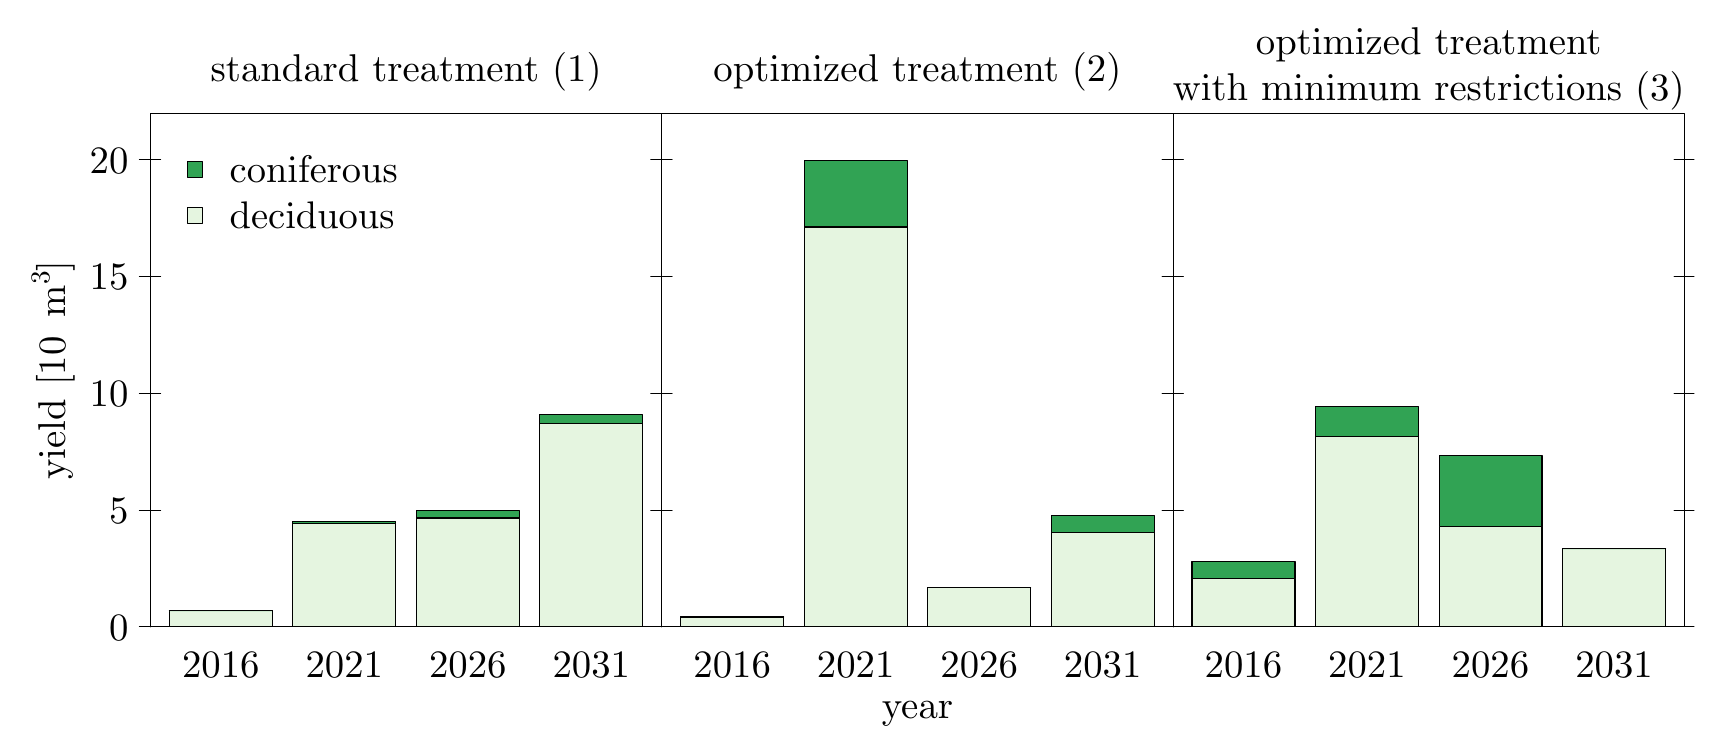
\begin{tikzpicture}[x=1pt,y=1pt]
\definecolor{fillColor}{RGB}{255,255,255}
\path[use as bounding box,fill=fillColor,fill opacity=0.00] (0,0) rectangle (602.23,252.94);
\begin{scope}
\path[clip] ( 44.35, 36.43) rectangle (229.12,222.06);
\definecolor{drawColor}{RGB}{0,0,0}
\definecolor{fillColor}{RGB}{229,245,224}

\path[draw=drawColor,line width= 0.4pt,line join=round,line cap=round,fill=fillColor] ( 51.20, 36.43) rectangle ( 88.39, 42.31);
\definecolor{fillColor}{RGB}{49,163,84}

\path[draw=drawColor,line width= 0.4pt,line join=round,line cap=round,fill=fillColor] ( 51.20, 42.31) rectangle ( 88.39, 42.31);
\definecolor{fillColor}{RGB}{229,245,224}

\path[draw=drawColor,line width= 0.4pt,line join=round,line cap=round,fill=fillColor] ( 95.83, 36.43) rectangle (133.02, 73.67);
\definecolor{fillColor}{RGB}{49,163,84}

\path[draw=drawColor,line width= 0.4pt,line join=round,line cap=round,fill=fillColor] ( 95.83, 73.67) rectangle (133.02, 74.64);
\definecolor{fillColor}{RGB}{229,245,224}

\path[draw=drawColor,line width= 0.4pt,line join=round,line cap=round,fill=fillColor] (140.46, 36.43) rectangle (177.65, 75.75);
\definecolor{fillColor}{RGB}{49,163,84}

\path[draw=drawColor,line width= 0.4pt,line join=round,line cap=round,fill=fillColor] (140.46, 75.75) rectangle (177.65, 78.43);
\definecolor{fillColor}{RGB}{229,245,224}

\path[draw=drawColor,line width= 0.4pt,line join=round,line cap=round,fill=fillColor] (185.09, 36.43) rectangle (222.28,109.94);
\definecolor{fillColor}{RGB}{49,163,84}

\path[draw=drawColor,line width= 0.4pt,line join=round,line cap=round,fill=fillColor] (185.09,109.94) rectangle (222.28,113.09);
\end{scope}
\begin{scope}
\path[clip] (  0.00,  0.00) rectangle (602.23,252.94);
\definecolor{drawColor}{RGB}{0,0,0}

\node[text=drawColor,anchor=base,inner sep=0pt, outer sep=0pt, scale=  1.40] at (136.74,233.66) {standard treatment (1)};

\path[draw=drawColor,line width= 0.4pt,line join=round,line cap=round] ( 44.35, 36.43) -- ( 40.39, 36.43);

\path[draw=drawColor,line width= 0.4pt,line join=round,line cap=round] ( 44.35, 78.62) -- ( 40.39, 78.62);

\path[draw=drawColor,line width= 0.4pt,line join=round,line cap=round] ( 44.35,120.81) -- ( 40.39,120.81);

\path[draw=drawColor,line width= 0.4pt,line join=round,line cap=round] ( 44.35,162.99) -- ( 40.39,162.99);

\path[draw=drawColor,line width= 0.4pt,line join=round,line cap=round] ( 44.35,205.18) -- ( 40.39,205.18);

\node[text=drawColor,anchor=base east,inner sep=0pt, outer sep=0pt, scale=  1.40] at ( 36.43, 31.61) {0};

\node[text=drawColor,anchor=base east,inner sep=0pt, outer sep=0pt, scale=  1.40] at ( 36.43, 73.80) {5};

\node[text=drawColor,anchor=base east,inner sep=0pt, outer sep=0pt, scale=  1.40] at ( 36.43,115.99) {10};

\node[text=drawColor,anchor=base east,inner sep=0pt, outer sep=0pt, scale=  1.40] at ( 36.43,158.17) {15};

\node[text=drawColor,anchor=base east,inner sep=0pt, outer sep=0pt, scale=  1.40] at ( 36.43,200.36) {20};

\path[draw=drawColor,line width= 0.4pt,line join=round,line cap=round] ( 44.35, 36.43) -- ( 48.05, 36.43);

\path[draw=drawColor,line width= 0.4pt,line join=round,line cap=round] ( 44.35, 78.62) -- ( 48.05, 78.62);

\path[draw=drawColor,line width= 0.4pt,line join=round,line cap=round] ( 44.35,120.81) -- ( 48.05,120.81);

\path[draw=drawColor,line width= 0.4pt,line join=round,line cap=round] ( 44.35,162.99) -- ( 48.05,162.99);

\path[draw=drawColor,line width= 0.4pt,line join=round,line cap=round] ( 44.35,205.18) -- ( 48.05,205.18);

\node[text=drawColor,anchor=base,inner sep=0pt, outer sep=0pt, scale=  1.40] at ( 69.79, 18.22) {2016};

\node[text=drawColor,anchor=base,inner sep=0pt, outer sep=0pt, scale=  1.40] at (114.42, 18.22) {2021};

\node[text=drawColor,anchor=base,inner sep=0pt, outer sep=0pt, scale=  1.40] at (159.05, 18.22) {2026};

\node[text=drawColor,anchor=base,inner sep=0pt, outer sep=0pt, scale=  1.40] at (203.68, 18.22) {2031};

\node[text=drawColor,rotate= 90.00,anchor=base west,inner sep=0pt, outer sep=0pt, scale=  1.40] at ( 13.53, 89.67) {yield [10};

\node[text=drawColor,rotate= 90.00,anchor=base west,inner sep=0pt, outer sep=0pt, scale=  1.40] at ( 13.53,141.37) { };

\node[text=drawColor,rotate= 90.00,anchor=base west,inner sep=0pt, outer sep=0pt, scale=  1.40] at ( 13.53,148.37) {m};

\node[text=drawColor,rotate= 90.00,anchor=base west,inner sep=0pt, outer sep=0pt, scale=  0.98] at (  7.80,160.04) {3};

\node[text=drawColor,rotate= 90.00,anchor=base west,inner sep=0pt, outer sep=0pt, scale=  1.40] at ( 13.53,164.94) {]};
\end{scope}
\begin{scope}
\path[clip] ( 44.35, 36.43) rectangle (229.12,222.06);
\definecolor{drawColor}{RGB}{0,0,0}
\definecolor{fillColor}{RGB}{49,163,84}

\path[draw=drawColor,line width= 0.4pt,line join=round,line cap=round,fill=fillColor] ( 57.76,198.95) rectangle ( 63.29,204.48);
\definecolor{fillColor}{RGB}{229,245,224}

\path[draw=drawColor,line width= 0.4pt,line join=round,line cap=round,fill=fillColor] ( 57.76,182.32) rectangle ( 63.29,187.84);

\node[text=drawColor,anchor=base west,inner sep=0pt, outer sep=0pt, scale=  1.39] at ( 73.00,196.94) {coniferous};

\node[text=drawColor,anchor=base west,inner sep=0pt, outer sep=0pt, scale=  1.39] at ( 73.00,180.31) {deciduous};
\end{scope}
\begin{scope}
\path[clip] (  0.00,  0.00) rectangle (602.23,252.94);
\definecolor{drawColor}{RGB}{0,0,0}

\path[draw=drawColor,line width= 0.4pt,line join=round,line cap=round] ( 44.35, 36.43) --
	(229.12, 36.43) --
	(229.12,222.06) --
	( 44.35,222.06) --
	( 44.35, 36.43);
\end{scope}
\begin{scope}
\path[clip] (229.12, 36.43) rectangle (413.89,222.06);
\definecolor{drawColor}{RGB}{0,0,0}
\definecolor{fillColor}{RGB}{229,245,224}

\path[draw=drawColor,line width= 0.4pt,line join=round,line cap=round,fill=fillColor] (235.97, 36.43) rectangle (273.16, 39.99);
\definecolor{fillColor}{RGB}{49,163,84}

\path[draw=drawColor,line width= 0.4pt,line join=round,line cap=round,fill=fillColor] (235.97, 39.99) rectangle (273.16, 39.99);
\definecolor{fillColor}{RGB}{229,245,224}

\path[draw=drawColor,line width= 0.4pt,line join=round,line cap=round,fill=fillColor] (280.60, 36.43) rectangle (317.79,180.91);
\definecolor{fillColor}{RGB}{49,163,84}

\path[draw=drawColor,line width= 0.4pt,line join=round,line cap=round,fill=fillColor] (280.60,180.91) rectangle (317.79,204.90);
\definecolor{fillColor}{RGB}{229,245,224}

\path[draw=drawColor,line width= 0.4pt,line join=round,line cap=round,fill=fillColor] (325.23, 36.43) rectangle (362.42, 50.69);
\definecolor{fillColor}{RGB}{49,163,84}

\path[draw=drawColor,line width= 0.4pt,line join=round,line cap=round,fill=fillColor] (325.23, 50.69) rectangle (362.42, 50.69);
\definecolor{fillColor}{RGB}{229,245,224}

\path[draw=drawColor,line width= 0.4pt,line join=round,line cap=round,fill=fillColor] (369.86, 36.43) rectangle (407.05, 70.62);
\definecolor{fillColor}{RGB}{49,163,84}

\path[draw=drawColor,line width= 0.4pt,line join=round,line cap=round,fill=fillColor] (369.86, 70.62) rectangle (407.05, 76.80);
\end{scope}
\begin{scope}
\path[clip] (  0.00,  0.00) rectangle (602.23,252.94);
\definecolor{drawColor}{RGB}{0,0,0}

\path[draw=drawColor,line width= 0.4pt,line join=round,line cap=round] (229.12, 36.43) -- (225.16, 36.43);

\path[draw=drawColor,line width= 0.4pt,line join=round,line cap=round] (229.12, 78.62) -- (225.16, 78.62);

\path[draw=drawColor,line width= 0.4pt,line join=round,line cap=round] (229.12,120.81) -- (225.16,120.81);

\path[draw=drawColor,line width= 0.4pt,line join=round,line cap=round] (229.12,162.99) -- (225.16,162.99);

\path[draw=drawColor,line width= 0.4pt,line join=round,line cap=round] (229.12,205.18) -- (225.16,205.18);

\path[draw=drawColor,line width= 0.4pt,line join=round,line cap=round] (229.12, 36.43) -- (232.82, 36.43);

\path[draw=drawColor,line width= 0.4pt,line join=round,line cap=round] (229.12, 78.62) -- (232.82, 78.62);

\path[draw=drawColor,line width= 0.4pt,line join=round,line cap=round] (229.12,120.81) -- (232.82,120.81);

\path[draw=drawColor,line width= 0.4pt,line join=round,line cap=round] (229.12,162.99) -- (232.82,162.99);

\path[draw=drawColor,line width= 0.4pt,line join=round,line cap=round] (229.12,205.18) -- (232.82,205.18);

\node[text=drawColor,anchor=base,inner sep=0pt, outer sep=0pt, scale=  1.40] at (254.56, 18.22) {2016};

\node[text=drawColor,anchor=base,inner sep=0pt, outer sep=0pt, scale=  1.40] at (299.19, 18.22) {2021};

\node[text=drawColor,anchor=base,inner sep=0pt, outer sep=0pt, scale=  1.40] at (343.82, 18.22) {2026};

\node[text=drawColor,anchor=base,inner sep=0pt, outer sep=0pt, scale=  1.40] at (388.45, 18.22) {2031};

\path[draw=drawColor,line width= 0.4pt,line join=round,line cap=round] (229.12, 36.43) --
	(413.89, 36.43) --
	(413.89,222.06) --
	(229.12,222.06) --
	(229.12, 36.43);

\node[text=drawColor,anchor=base,inner sep=0pt, outer sep=0pt, scale=  1.40] at (321.51,233.66) {optimized treatment (2)};

\node[text=drawColor,anchor=base,inner sep=0pt, outer sep=0pt, scale=  1.40] at (321.51,  3.17) {year};
\end{scope}
\begin{scope}
\path[clip] (413.89, 36.43) rectangle (598.66,222.06);
\definecolor{drawColor}{RGB}{0,0,0}
\definecolor{fillColor}{RGB}{229,245,224}

\path[draw=drawColor,line width= 0.4pt,line join=round,line cap=round,fill=fillColor] (420.74, 36.43) rectangle (457.93, 53.86);
\definecolor{fillColor}{RGB}{49,163,84}

\path[draw=drawColor,line width= 0.4pt,line join=round,line cap=round,fill=fillColor] (420.74, 53.86) rectangle (457.93, 59.96);
\definecolor{fillColor}{RGB}{229,245,224}

\path[draw=drawColor,line width= 0.4pt,line join=round,line cap=round,fill=fillColor] (465.37, 36.43) rectangle (502.56,105.28);
\definecolor{fillColor}{RGB}{49,163,84}

\path[draw=drawColor,line width= 0.4pt,line join=round,line cap=round,fill=fillColor] (465.37,105.28) rectangle (502.56,116.05);
\definecolor{fillColor}{RGB}{229,245,224}

\path[draw=drawColor,line width= 0.4pt,line join=round,line cap=round,fill=fillColor] (510.00, 36.43) rectangle (547.19, 72.60);
\definecolor{fillColor}{RGB}{49,163,84}

\path[draw=drawColor,line width= 0.4pt,line join=round,line cap=round,fill=fillColor] (510.00, 72.60) rectangle (547.19, 98.36);
\definecolor{fillColor}{RGB}{229,245,224}

\path[draw=drawColor,line width= 0.4pt,line join=round,line cap=round,fill=fillColor] (554.63, 36.43) rectangle (591.82, 64.58);
\definecolor{fillColor}{RGB}{49,163,84}

\path[draw=drawColor,line width= 0.4pt,line join=round,line cap=round,fill=fillColor] (554.63, 64.58) rectangle (591.82, 64.58);
\end{scope}
\begin{scope}
\path[clip] (  0.00,  0.00) rectangle (602.23,252.94);
\definecolor{drawColor}{RGB}{0,0,0}

\path[draw=drawColor,line width= 0.4pt,line join=round,line cap=round] (413.89, 36.43) -- (409.93, 36.43);

\path[draw=drawColor,line width= 0.4pt,line join=round,line cap=round] (413.89, 78.62) -- (409.93, 78.62);

\path[draw=drawColor,line width= 0.4pt,line join=round,line cap=round] (413.89,120.81) -- (409.93,120.81);

\path[draw=drawColor,line width= 0.4pt,line join=round,line cap=round] (413.89,162.99) -- (409.93,162.99);

\path[draw=drawColor,line width= 0.4pt,line join=round,line cap=round] (413.89,205.18) -- (409.93,205.18);

\path[draw=drawColor,line width= 0.4pt,line join=round,line cap=round] (413.89, 36.43) -- (417.59, 36.43);

\path[draw=drawColor,line width= 0.4pt,line join=round,line cap=round] (413.89, 78.62) -- (417.59, 78.62);

\path[draw=drawColor,line width= 0.4pt,line join=round,line cap=round] (413.89,120.81) -- (417.59,120.81);

\path[draw=drawColor,line width= 0.4pt,line join=round,line cap=round] (413.89,162.99) -- (417.59,162.99);

\path[draw=drawColor,line width= 0.4pt,line join=round,line cap=round] (413.89,205.18) -- (417.59,205.18);

\path[draw=drawColor,line width= 0.4pt,line join=round,line cap=round] (598.66, 36.43) -- (602.23, 36.43);

\path[draw=drawColor,line width= 0.4pt,line join=round,line cap=round] (598.66, 78.62) -- (602.23, 78.62);

\path[draw=drawColor,line width= 0.4pt,line join=round,line cap=round] (598.66,120.81) -- (602.23,120.81);

\path[draw=drawColor,line width= 0.4pt,line join=round,line cap=round] (598.66,162.99) -- (602.23,162.99);

\path[draw=drawColor,line width= 0.4pt,line join=round,line cap=round] (598.66,205.18) -- (602.23,205.18);

\path[draw=drawColor,line width= 0.4pt,line join=round,line cap=round] (598.66, 36.43) -- (594.97, 36.43);

\path[draw=drawColor,line width= 0.4pt,line join=round,line cap=round] (598.66, 78.62) -- (594.97, 78.62);

\path[draw=drawColor,line width= 0.4pt,line join=round,line cap=round] (598.66,120.81) -- (594.97,120.81);

\path[draw=drawColor,line width= 0.4pt,line join=round,line cap=round] (598.66,162.99) -- (594.97,162.99);

\path[draw=drawColor,line width= 0.4pt,line join=round,line cap=round] (598.66,205.18) -- (594.97,205.18);

\node[text=drawColor,anchor=base,inner sep=0pt, outer sep=0pt, scale=  1.40] at (439.33, 18.22) {2016};

\node[text=drawColor,anchor=base,inner sep=0pt, outer sep=0pt, scale=  1.40] at (483.96, 18.22) {2021};

\node[text=drawColor,anchor=base,inner sep=0pt, outer sep=0pt, scale=  1.40] at (528.59, 18.22) {2026};

\node[text=drawColor,anchor=base,inner sep=0pt, outer sep=0pt, scale=  1.40] at (573.22, 18.22) {2031};

\node[text=drawColor,anchor=base,inner sep=0pt, outer sep=0pt, scale=  1.40] at (506.28,243.30) {optimized treatment};

\node[text=drawColor,anchor=base,inner sep=0pt, outer sep=0pt, scale=  1.40] at (506.28,226.50) {with minimum restrictions (3)};

\path[draw=drawColor,line width= 0.4pt,line join=round,line cap=round] (413.89, 36.43) --
	(598.66, 36.43) --
	(598.66,222.06) --
	(413.89,222.06) --
	(413.89, 36.43);
\end{scope}
\end{tikzpicture}
}
		\caption{Summed simulated yields of the first exemplary forest enterprise in five-year periods, beginning with the period from 2011 to 2016. The simulated yield amounts are differentiated into coniferous and deciduous wood volume (including bark).}
		\label{fig:discussion:fig1}
	\end{figure}
}

The simulated yields, though, differed substantially between the three scenarios (Figure \ref{fig:discussion:fig1}). Yielded wood volume from target usage was negligible in all scenarios. It showed up that intensive harvesting in the second time period is favorable in terms of total yields. The optimal enterprise-specific wood potential within the simulation period would be achieved, if the stands were treated intensively between 2016 and 2021. With an overall yield of 267 m$^3$, the wood potential of the optimized treatment scenario was 32 \% higher than the potential of the standard scenario. Extremely unbalanced stand treatments performed best in terms of the total wood potential. Cooperations between forest enterprises and bio-economy companies often involve continuous wood supply (Subsection \ref{subsec:intro:struct:opt}). So there are good reasons why forest enterprises and bio-economy could be interested in balanced yields. This was in contrast with the results from scenarios one and two because both scenarios forecasted only small wood potentials in at least one of the five-year time periods. If delivery contracts with balanced annual wood amounts were arranged, minimum harvesting restrictions would have been indispensable in the first exemplary forest enterprise. For this, minimum harvesting restriction for low-valued European beech wood from thinning activities were defined. The restriction amounted to 4 m$^3$ year$^{-1}$ (20 m$^3$ in the 5-year period). It had substantial influence on the optimal stand treatments. Figure \ref{fig:discussion:fig1} (right) shows that the minimum restriction led to homogeneous yields for the deciduous wood volumes. The deciduous harvesting volumes in the first time period, which was below the minimum restriction in each other scenario, amounted roughly the minimum restriction (20,7 m$^3$). This reveals that usage in the first 5-year period is, under given tree species and age combinations, not reasonable in terms of wood potential optimization. The restrictions are needed to force a usage in this period. The usages of trees in period 1 were, despite a few trees, ahead of the reasonable schedule. The tree-individual growth potential would not used, if the trees were used in the first period. A force to harvest them, of course, led to a reduction of the overall wood potential. The summed wood potential of the scenario three was 17 \% below the potential of the unrestricted scenario two. This difference in the wood potentials builds the basis for the calculation of the opportunity costs. They enable a differentiated, evidence-based trade-off between advantages and drawbacks of delivery contracts. In the example, the matching of continuous wood demands reduced the total available wood potential by 40 m$^3$. Forest owners could decide whether the advantages in the intermediate-term planning, that a delivery contract entailed, justified opportunity costs of 40 m$^3$.

\textsc{\begin{figure}[h]
		\center
		\resizebox{.6\linewidth}{!}{% Created by tikzDevice version 0.10.1 on 2017-05-27 13:39:00
% !TEX encoding = UTF-8 Unicode
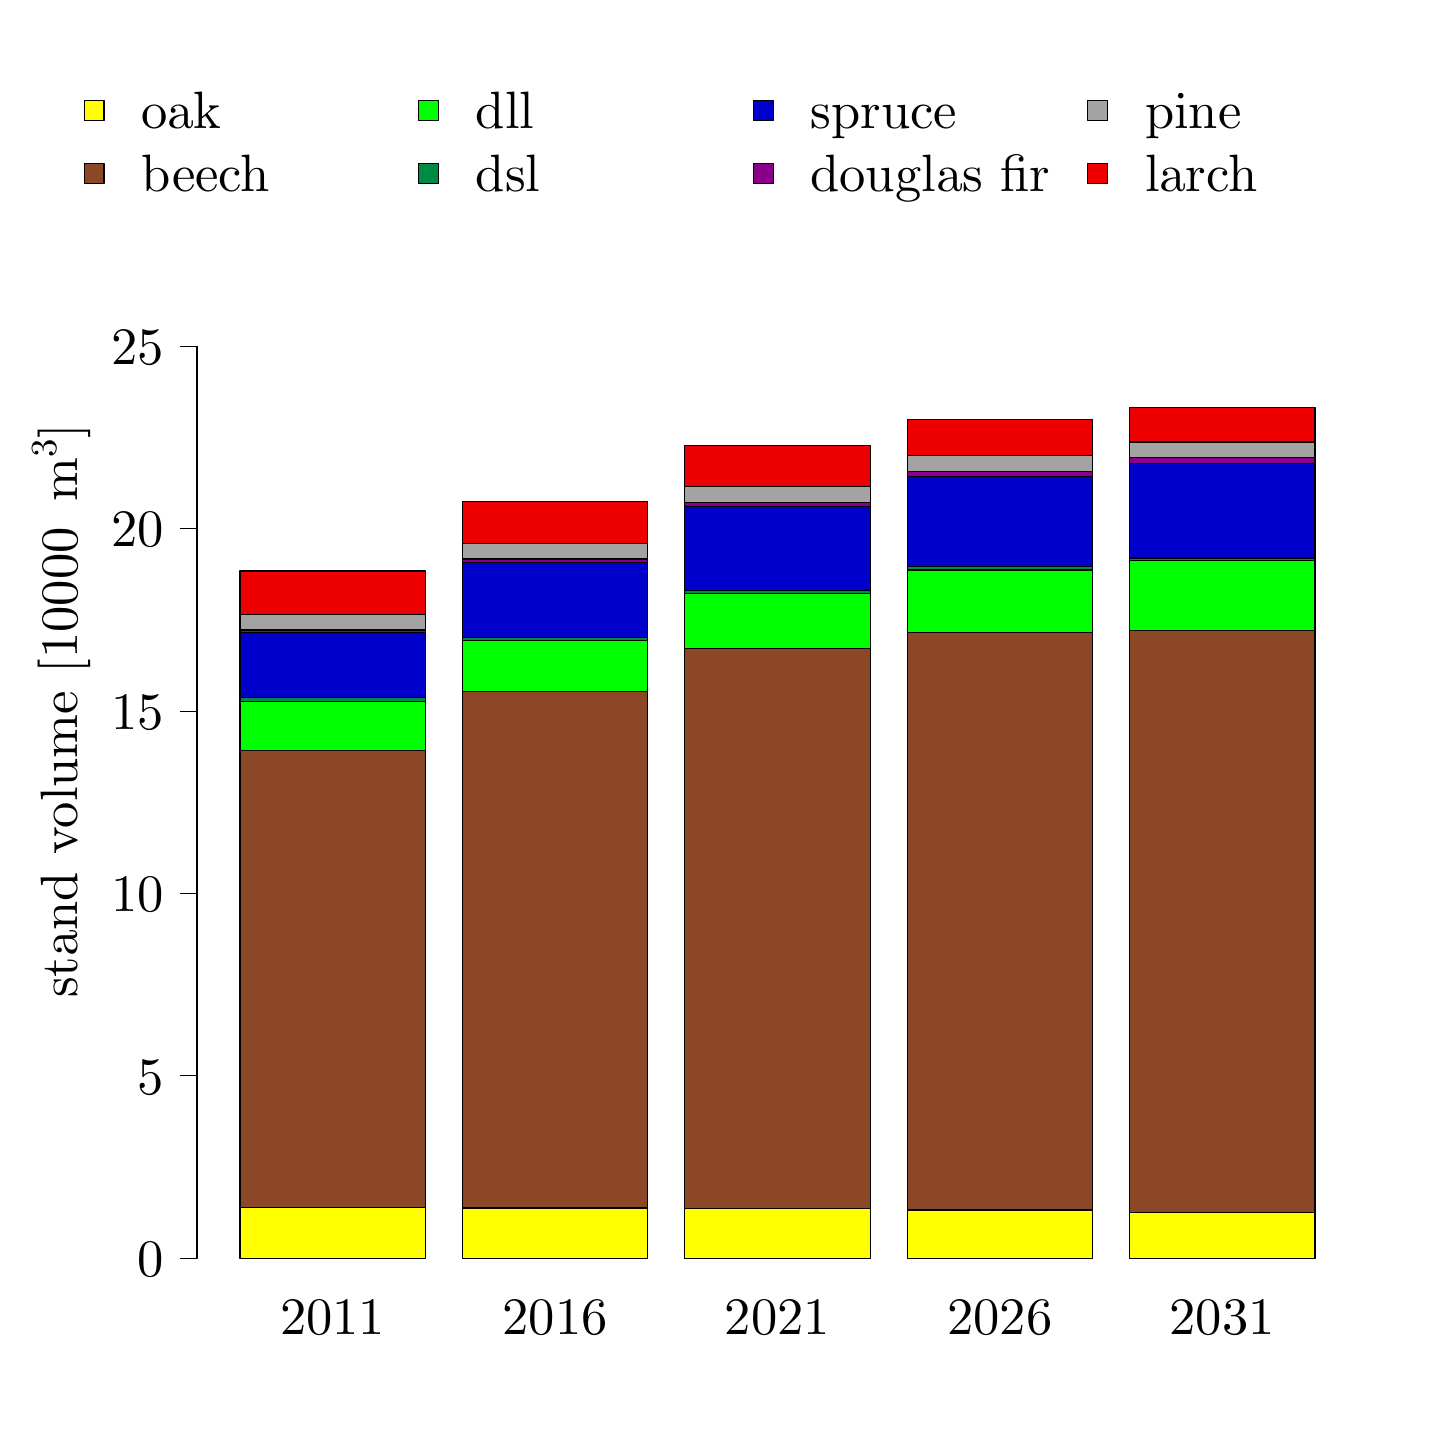
\begin{tikzpicture}[x=1pt,y=1pt]
\definecolor{fillColor}{RGB}{255,255,255}
\path[use as bounding box,fill=fillColor,fill opacity=0.00] (0,0) rectangle (505.89,505.89);
\begin{scope}
\path[clip] (  0.00,  0.00) rectangle (505.89,505.89);
\definecolor{drawColor}{RGB}{0,0,0}
\definecolor{fillColor}{RGB}{255,255,0}

\path[draw=drawColor,line width= 0.4pt,line join=round,line cap=round,fill=fillColor] ( 76.74, 61.20) rectangle (143.71, 79.52);
\definecolor{fillColor}{RGB}{139,71,38}

\path[draw=drawColor,line width= 0.4pt,line join=round,line cap=round,fill=fillColor] ( 76.74, 79.52) rectangle (143.71,244.80);
\definecolor{fillColor}{RGB}{0,255,0}

\path[draw=drawColor,line width= 0.4pt,line join=round,line cap=round,fill=fillColor] ( 76.74,244.80) rectangle (143.71,262.30);
\definecolor{fillColor}{RGB}{0,139,69}

\path[draw=drawColor,line width= 0.4pt,line join=round,line cap=round,fill=fillColor] ( 76.74,262.30) rectangle (143.71,263.78);
\definecolor{fillColor}{RGB}{0,0,205}

\path[draw=drawColor,line width= 0.4pt,line join=round,line cap=round,fill=fillColor] ( 76.74,263.78) rectangle (143.71,287.35);
\definecolor{fillColor}{RGB}{139,0,139}

\path[draw=drawColor,line width= 0.4pt,line join=round,line cap=round,fill=fillColor] ( 76.74,287.35) rectangle (143.71,288.25);
\definecolor{fillColor}{gray}{0.64}

\path[draw=drawColor,line width= 0.4pt,line join=round,line cap=round,fill=fillColor] ( 76.74,288.25) rectangle (143.71,293.71);
\definecolor{fillColor}{RGB}{238,0,0}

\path[draw=drawColor,line width= 0.4pt,line join=round,line cap=round,fill=fillColor] ( 76.74,293.71) rectangle (143.71,309.54);
\definecolor{fillColor}{RGB}{255,255,0}

\path[draw=drawColor,line width= 0.4pt,line join=round,line cap=round,fill=fillColor] (157.10, 61.20) rectangle (224.07, 79.39);
\definecolor{fillColor}{RGB}{139,71,38}

\path[draw=drawColor,line width= 0.4pt,line join=round,line cap=round,fill=fillColor] (157.10, 79.39) rectangle (224.07,266.07);
\definecolor{fillColor}{RGB}{0,255,0}

\path[draw=drawColor,line width= 0.4pt,line join=round,line cap=round,fill=fillColor] (157.10,266.07) rectangle (224.07,284.30);
\definecolor{fillColor}{RGB}{0,139,69}

\path[draw=drawColor,line width= 0.4pt,line join=round,line cap=round,fill=fillColor] (157.10,284.30) rectangle (224.07,285.42);
\definecolor{fillColor}{RGB}{0,0,205}

\path[draw=drawColor,line width= 0.4pt,line join=round,line cap=round,fill=fillColor] (157.10,285.42) rectangle (224.07,312.71);
\definecolor{fillColor}{RGB}{139,0,139}

\path[draw=drawColor,line width= 0.4pt,line join=round,line cap=round,fill=fillColor] (157.10,312.71) rectangle (224.07,313.89);
\definecolor{fillColor}{gray}{0.64}

\path[draw=drawColor,line width= 0.4pt,line join=round,line cap=round,fill=fillColor] (157.10,313.89) rectangle (224.07,319.39);
\definecolor{fillColor}{RGB}{238,0,0}

\path[draw=drawColor,line width= 0.4pt,line join=round,line cap=round,fill=fillColor] (157.10,319.39) rectangle (224.07,334.69);
\definecolor{fillColor}{RGB}{255,255,0}

\path[draw=drawColor,line width= 0.4pt,line join=round,line cap=round,fill=fillColor] (237.46, 61.20) rectangle (304.43, 79.21);
\definecolor{fillColor}{RGB}{139,71,38}

\path[draw=drawColor,line width= 0.4pt,line join=round,line cap=round,fill=fillColor] (237.46, 79.21) rectangle (304.43,281.55);
\definecolor{fillColor}{RGB}{0,255,0}

\path[draw=drawColor,line width= 0.4pt,line join=round,line cap=round,fill=fillColor] (237.46,281.55) rectangle (304.43,301.29);
\definecolor{fillColor}{RGB}{0,139,69}

\path[draw=drawColor,line width= 0.4pt,line join=round,line cap=round,fill=fillColor] (237.46,301.29) rectangle (304.43,302.52);
\definecolor{fillColor}{RGB}{0,0,205}

\path[draw=drawColor,line width= 0.4pt,line join=round,line cap=round,fill=fillColor] (237.46,302.52) rectangle (304.43,332.85);
\definecolor{fillColor}{RGB}{139,0,139}

\path[draw=drawColor,line width= 0.4pt,line join=round,line cap=round,fill=fillColor] (237.46,332.85) rectangle (304.43,334.29);
\definecolor{fillColor}{gray}{0.64}

\path[draw=drawColor,line width= 0.4pt,line join=round,line cap=round,fill=fillColor] (237.46,334.29) rectangle (304.43,340.02);
\definecolor{fillColor}{RGB}{238,0,0}

\path[draw=drawColor,line width= 0.4pt,line join=round,line cap=round,fill=fillColor] (237.46,340.02) rectangle (304.43,354.75);
\definecolor{fillColor}{RGB}{255,255,0}

\path[draw=drawColor,line width= 0.4pt,line join=round,line cap=round,fill=fillColor] (317.82, 61.20) rectangle (384.79, 78.67);
\definecolor{fillColor}{RGB}{139,71,38}

\path[draw=drawColor,line width= 0.4pt,line join=round,line cap=round,fill=fillColor] (317.82, 78.67) rectangle (384.79,287.42);
\definecolor{fillColor}{RGB}{0,255,0}

\path[draw=drawColor,line width= 0.4pt,line join=round,line cap=round,fill=fillColor] (317.82,287.42) rectangle (384.79,309.93);
\definecolor{fillColor}{RGB}{0,139,69}

\path[draw=drawColor,line width= 0.4pt,line join=round,line cap=round,fill=fillColor] (317.82,309.93) rectangle (384.79,311.11);
\definecolor{fillColor}{RGB}{0,0,205}

\path[draw=drawColor,line width= 0.4pt,line join=round,line cap=round,fill=fillColor] (317.82,311.11) rectangle (384.79,343.72);
\definecolor{fillColor}{RGB}{139,0,139}

\path[draw=drawColor,line width= 0.4pt,line join=round,line cap=round,fill=fillColor] (317.82,343.72) rectangle (384.79,345.62);
\definecolor{fillColor}{gray}{0.64}

\path[draw=drawColor,line width= 0.4pt,line join=round,line cap=round,fill=fillColor] (317.82,345.62) rectangle (384.79,351.22);
\definecolor{fillColor}{RGB}{238,0,0}

\path[draw=drawColor,line width= 0.4pt,line join=round,line cap=round,fill=fillColor] (317.82,351.22) rectangle (384.79,364.22);
\definecolor{fillColor}{RGB}{255,255,0}

\path[draw=drawColor,line width= 0.4pt,line join=round,line cap=round,fill=fillColor] (398.18, 61.20) rectangle (465.15, 77.89);
\definecolor{fillColor}{RGB}{139,71,38}

\path[draw=drawColor,line width= 0.4pt,line join=round,line cap=round,fill=fillColor] (398.18, 77.89) rectangle (465.15,288.16);
\definecolor{fillColor}{RGB}{0,255,0}

\path[draw=drawColor,line width= 0.4pt,line join=round,line cap=round,fill=fillColor] (398.18,288.16) rectangle (465.15,313.24);
\definecolor{fillColor}{RGB}{0,139,69}

\path[draw=drawColor,line width= 0.4pt,line join=round,line cap=round,fill=fillColor] (398.18,313.24) rectangle (465.15,314.25);
\definecolor{fillColor}{RGB}{0,0,205}

\path[draw=drawColor,line width= 0.4pt,line join=round,line cap=round,fill=fillColor] (398.18,314.25) rectangle (465.15,348.56);
\definecolor{fillColor}{RGB}{139,0,139}

\path[draw=drawColor,line width= 0.4pt,line join=round,line cap=round,fill=fillColor] (398.18,348.56) rectangle (465.15,350.57);
\definecolor{fillColor}{gray}{0.64}

\path[draw=drawColor,line width= 0.4pt,line join=round,line cap=round,fill=fillColor] (398.18,350.57) rectangle (465.15,356.15);
\definecolor{fillColor}{RGB}{238,0,0}

\path[draw=drawColor,line width= 0.4pt,line join=round,line cap=round,fill=fillColor] (398.18,356.15) rectangle (465.15,368.68);
\end{scope}
\begin{scope}
\path[clip] (  0.00,  0.00) rectangle (505.89,505.89);
\definecolor{drawColor}{RGB}{0,0,0}

\node[text=drawColor,rotate= 90.00,anchor=base west,inner sep=0pt, outer sep=0pt, scale=  1.90] at ( 18.05,155.32) {stand volume [10000};

\node[text=drawColor,rotate= 90.00,anchor=base west,inner sep=0pt, outer sep=0pt, scale=  1.90] at ( 18.05,325.32) { };

\node[text=drawColor,rotate= 90.00,anchor=base west,inner sep=0pt, outer sep=0pt, scale=  1.90] at ( 18.05,334.82) {m};

\node[text=drawColor,rotate= 90.00,anchor=base west,inner sep=0pt, outer sep=0pt, scale=  1.33] at ( 10.28,350.65) {3};

\node[text=drawColor,rotate= 90.00,anchor=base west,inner sep=0pt, outer sep=0pt, scale=  1.90] at ( 18.05,357.30) {]};

\node[text=drawColor,anchor=base,inner sep=0pt, outer sep=0pt, scale=  1.90] at (110.22, 33.60) {2011};

\node[text=drawColor,anchor=base,inner sep=0pt, outer sep=0pt, scale=  1.90] at (190.58, 33.60) {2016};

\node[text=drawColor,anchor=base,inner sep=0pt, outer sep=0pt, scale=  1.90] at (270.94, 33.60) {2021};

\node[text=drawColor,anchor=base,inner sep=0pt, outer sep=0pt, scale=  1.90] at (351.31, 33.60) {2026};

\node[text=drawColor,anchor=base,inner sep=0pt, outer sep=0pt, scale=  1.90] at (431.67, 33.60) {2031};

\path[draw=drawColor,line width= 0.4pt,line join=round,line cap=round] ( 61.20, 61.20) -- ( 61.20,390.78);

\path[draw=drawColor,line width= 0.4pt,line join=round,line cap=round] ( 61.20, 61.20) -- ( 55.20, 61.20);

\path[draw=drawColor,line width= 0.4pt,line join=round,line cap=round] ( 61.20,127.11) -- ( 55.20,127.11);

\path[draw=drawColor,line width= 0.4pt,line join=round,line cap=round] ( 61.20,193.03) -- ( 55.20,193.03);

\path[draw=drawColor,line width= 0.4pt,line join=round,line cap=round] ( 61.20,258.94) -- ( 55.20,258.94);

\path[draw=drawColor,line width= 0.4pt,line join=round,line cap=round] ( 61.20,324.86) -- ( 55.20,324.86);

\path[draw=drawColor,line width= 0.4pt,line join=round,line cap=round] ( 61.20,390.78) -- ( 55.20,390.78);

\node[text=drawColor,anchor=base east,inner sep=0pt, outer sep=0pt, scale=  1.90] at ( 49.20, 54.66) {0};

\node[text=drawColor,anchor=base east,inner sep=0pt, outer sep=0pt, scale=  1.90] at ( 49.20,120.57) {5};

\node[text=drawColor,anchor=base east,inner sep=0pt, outer sep=0pt, scale=  1.90] at ( 49.20,186.49) {10};

\node[text=drawColor,anchor=base east,inner sep=0pt, outer sep=0pt, scale=  1.90] at ( 49.20,252.40) {15};

\node[text=drawColor,anchor=base east,inner sep=0pt, outer sep=0pt, scale=  1.90] at ( 49.20,318.32) {20};

\node[text=drawColor,anchor=base east,inner sep=0pt, outer sep=0pt, scale=  1.90] at ( 49.20,384.23) {25};
\end{scope}
\begin{scope}
\path[clip] (  1.20,  1.20) rectangle (504.69,498.69);
\definecolor{drawColor}{RGB}{0,0,0}
\definecolor{fillColor}{RGB}{255,255,0}

\path[draw=drawColor,line width= 0.4pt,line join=round,line cap=round,fill=fillColor] ( 20.40,472.30) rectangle ( 27.57,479.48);
\definecolor{fillColor}{RGB}{139,71,38}

\path[draw=drawColor,line width= 0.4pt,line join=round,line cap=round,fill=fillColor] ( 20.40,449.50) rectangle ( 27.57,456.68);
\definecolor{fillColor}{RGB}{0,255,0}

\path[draw=drawColor,line width= 0.4pt,line join=round,line cap=round,fill=fillColor] (141.29,472.30) rectangle (148.47,479.48);
\definecolor{fillColor}{RGB}{0,139,69}

\path[draw=drawColor,line width= 0.4pt,line join=round,line cap=round,fill=fillColor] (141.29,449.50) rectangle (148.47,456.68);
\definecolor{fillColor}{RGB}{0,0,205}

\path[draw=drawColor,line width= 0.4pt,line join=round,line cap=round,fill=fillColor] (262.18,472.30) rectangle (269.36,479.48);
\definecolor{fillColor}{RGB}{139,0,139}

\path[draw=drawColor,line width= 0.4pt,line join=round,line cap=round,fill=fillColor] (262.18,449.50) rectangle (269.36,456.68);
\definecolor{fillColor}{gray}{0.64}

\path[draw=drawColor,line width= 0.4pt,line join=round,line cap=round,fill=fillColor] (383.07,472.30) rectangle (390.25,479.48);
\definecolor{fillColor}{RGB}{238,0,0}

\path[draw=drawColor,line width= 0.4pt,line join=round,line cap=round,fill=fillColor] (383.07,449.50) rectangle (390.25,456.68);

\node[text=drawColor,anchor=base west,inner sep=0pt, outer sep=0pt, scale=  1.90] at ( 41.09,469.35) {oak};

\node[text=drawColor,anchor=base west,inner sep=0pt, outer sep=0pt, scale=  1.90] at ( 41.09,446.55) {beech};

\node[text=drawColor,anchor=base west,inner sep=0pt, outer sep=0pt, scale=  1.90] at (161.98,469.35) {dll};

\node[text=drawColor,anchor=base west,inner sep=0pt, outer sep=0pt, scale=  1.90] at (161.98,446.55) {dsl};

\node[text=drawColor,anchor=base west,inner sep=0pt, outer sep=0pt, scale=  1.90] at (282.87,469.35) {spruce};

\node[text=drawColor,anchor=base west,inner sep=0pt, outer sep=0pt, scale=  1.90] at (282.87,446.55) {douglas fir};

\node[text=drawColor,anchor=base west,inner sep=0pt, outer sep=0pt, scale=  1.90] at (403.76,469.35) {pine};

\node[text=drawColor,anchor=base west,inner sep=0pt, outer sep=0pt, scale=  1.90] at (403.76,446.55) {larch};
\end{scope}
\end{tikzpicture}
}
		\caption{Development of the summed stand volumes of all forest stands of the second exemplary forest enterprise. The forest stands were forecasted using the standard treatment settings without optimization (scenario one).}
		\label{fig:discussion:fig2}
	\end{figure}
}

As the second exemplary enterprise contained too many stands to evaluate each stand volume separately, the stand volumes are displayed in sums of tree species groups (Figure \ref{fig:discussion:fig2}). The stand volumes in the last simulated year of all three scenarios were very close, just as it was observed in the first example. The tree scenarios differed, again, in the allocation of the harvestable wood volumes but not in the stand volumes at the end of the simulations. It showed up that the growth, by trend, exceeds the usage. Especially for European beech, the summed stand volumes increased in the entire simulation period (Figure \ref{fig:discussion:fig2}). This reflects the typical stands developments in the forest district of Reinhausen \citep{nlf_2017}.

The results of the second exemplary enterprise (Figure \ref{fig:discussion:fig3}) were not as obvious as the results from in the first example (Figure \ref{fig:discussion:fig1}). With 78,527 m$^3$, the optimized treatment simulation led to 9 \% higher harvesting amounts than the standard treatment simulation during the entire simulation period. Only the potentials of deciduous thinning assortments in the third and fourth time periods differed between the scenarios. The evaluation of minimum harvesting volumes for deciduous thinning assortments uncovered two results. The first, and probably very interesting result for decision-makers, was that the harvesting volumes of deciduous thinning assortments of scenario 3 differed only very slightly from the scenario 2. The definition of minimum harvesting amounts for deciduous thinning assortments above 4,500 m$^3$ in five years (900 m$^3$ year$^{-1}$) did not lead to valid results. This means that minimum harvesting restrictions above 900 m$^3$ year$^{-1}$ would violate the implemented principle of sustainability. For comparison, the actual harvesting volume in scenario 2 was 838 m$^3$ year$^{-1}$. The difference in the overall wood potential were also slight between scenario 2 and 3 (1.5 \%). The only remarkable difference were found in the allocations of the yields in the time periods three and four. Those allocations had no remarkable influence on the overall wood potential. The optimized treatment hence already reflected the continuously available volume amount of deciduous thinning assortments.

\textsc{\begin{figure}[h]
		\center
		\resizebox{1\linewidth}{!}{% Created by tikzDevice version 0.10.1 on 2017-05-25 12:28:08
% !TEX encoding = UTF-8 Unicode
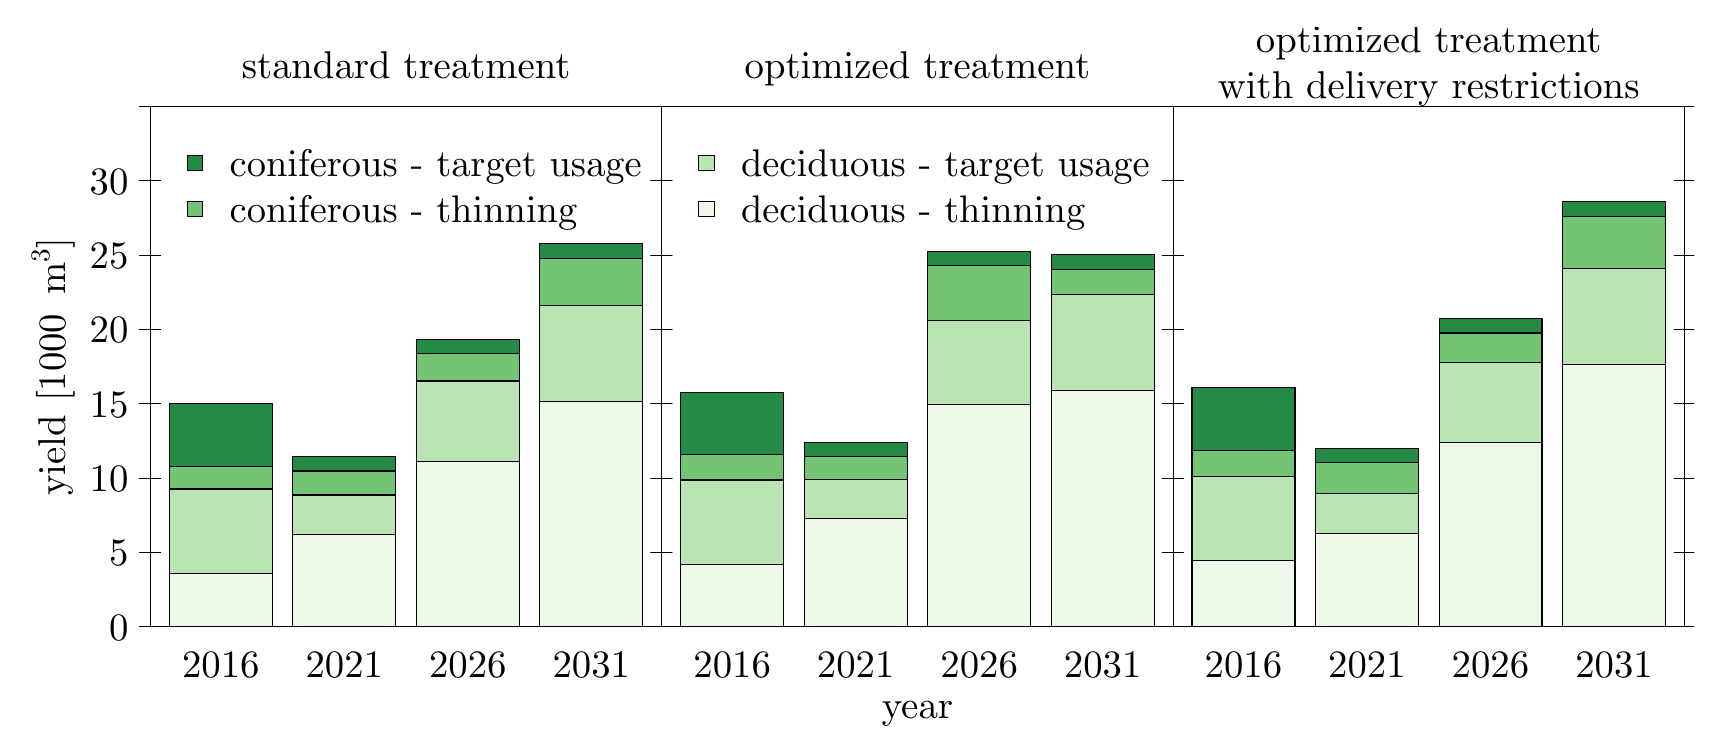
\begin{tikzpicture}[x=1pt,y=1pt]
\definecolor{fillColor}{RGB}{255,255,255}
\path[use as bounding box,fill=fillColor,fill opacity=0.00] (0,0) rectangle (602.23,252.94);
\begin{scope}
\path[clip] ( 44.35, 36.43) rectangle (229.12,224.43);
\definecolor{drawColor}{RGB}{0,0,0}
\definecolor{fillColor}{RGB}{237,248,233}

\path[draw=drawColor,line width= 0.4pt,line join=round,line cap=round,fill=fillColor] ( 51.20, 36.43) rectangle ( 88.39, 55.69);
\definecolor{fillColor}{RGB}{186,228,179}

\path[draw=drawColor,line width= 0.4pt,line join=round,line cap=round,fill=fillColor] ( 51.20, 55.69) rectangle ( 88.39, 86.24);
\definecolor{fillColor}{RGB}{116,196,118}

\path[draw=drawColor,line width= 0.4pt,line join=round,line cap=round,fill=fillColor] ( 51.20, 86.24) rectangle ( 88.39, 94.31);
\definecolor{fillColor}{RGB}{35,139,69}

\path[draw=drawColor,line width= 0.4pt,line join=round,line cap=round,fill=fillColor] ( 51.20, 94.31) rectangle ( 88.39,117.00);
\definecolor{fillColor}{RGB}{237,248,233}

\path[draw=drawColor,line width= 0.4pt,line join=round,line cap=round,fill=fillColor] ( 95.83, 36.43) rectangle (133.02, 69.72);
\definecolor{fillColor}{RGB}{186,228,179}

\path[draw=drawColor,line width= 0.4pt,line join=round,line cap=round,fill=fillColor] ( 95.83, 69.72) rectangle (133.02, 84.07);
\definecolor{fillColor}{RGB}{116,196,118}

\path[draw=drawColor,line width= 0.4pt,line join=round,line cap=round,fill=fillColor] ( 95.83, 84.07) rectangle (133.02, 92.74);
\definecolor{fillColor}{RGB}{35,139,69}

\path[draw=drawColor,line width= 0.4pt,line join=round,line cap=round,fill=fillColor] ( 95.83, 92.74) rectangle (133.02, 98.01);
\definecolor{fillColor}{RGB}{237,248,233}

\path[draw=drawColor,line width= 0.4pt,line join=round,line cap=round,fill=fillColor] (140.46, 36.43) rectangle (177.65, 96.30);
\definecolor{fillColor}{RGB}{186,228,179}

\path[draw=drawColor,line width= 0.4pt,line join=round,line cap=round,fill=fillColor] (140.46, 96.30) rectangle (177.65,125.25);
\definecolor{fillColor}{RGB}{116,196,118}

\path[draw=drawColor,line width= 0.4pt,line join=round,line cap=round,fill=fillColor] (140.46,125.25) rectangle (177.65,135.10);
\definecolor{fillColor}{RGB}{35,139,69}

\path[draw=drawColor,line width= 0.4pt,line join=round,line cap=round,fill=fillColor] (140.46,135.10) rectangle (177.65,140.36);
\definecolor{fillColor}{RGB}{237,248,233}

\path[draw=drawColor,line width= 0.4pt,line join=round,line cap=round,fill=fillColor] (185.09, 36.43) rectangle (222.28,117.84);
\definecolor{fillColor}{RGB}{186,228,179}

\path[draw=drawColor,line width= 0.4pt,line join=round,line cap=round,fill=fillColor] (185.09,117.84) rectangle (222.28,152.47);
\definecolor{fillColor}{RGB}{116,196,118}

\path[draw=drawColor,line width= 0.4pt,line join=round,line cap=round,fill=fillColor] (185.09,152.47) rectangle (222.28,169.50);
\definecolor{fillColor}{RGB}{35,139,69}

\path[draw=drawColor,line width= 0.4pt,line join=round,line cap=round,fill=fillColor] (185.09,169.50) rectangle (222.28,174.87);
\end{scope}
\begin{scope}
\path[clip] (  0.00,  0.00) rectangle (602.23,252.94);
\definecolor{drawColor}{RGB}{0,0,0}

\node[text=drawColor,anchor=base,inner sep=0pt, outer sep=0pt, scale=  1.40] at (136.74,234.45) {standard treatment};

\path[draw=drawColor,line width= 0.4pt,line join=round,line cap=round] ( 44.35, 36.43) -- ( 40.39, 36.43);

\path[draw=drawColor,line width= 0.4pt,line join=round,line cap=round] ( 44.35, 63.29) -- ( 40.39, 63.29);

\path[draw=drawColor,line width= 0.4pt,line join=round,line cap=round] ( 44.35, 90.15) -- ( 40.39, 90.15);

\path[draw=drawColor,line width= 0.4pt,line join=round,line cap=round] ( 44.35,117.00) -- ( 40.39,117.00);

\path[draw=drawColor,line width= 0.4pt,line join=round,line cap=round] ( 44.35,143.86) -- ( 40.39,143.86);

\path[draw=drawColor,line width= 0.4pt,line join=round,line cap=round] ( 44.35,170.72) -- ( 40.39,170.72);

\path[draw=drawColor,line width= 0.4pt,line join=round,line cap=round] ( 44.35,197.58) -- ( 40.39,197.58);

\path[draw=drawColor,line width= 0.4pt,line join=round,line cap=round] ( 44.35,224.43) -- ( 40.39,224.43);

\node[text=drawColor,anchor=base east,inner sep=0pt, outer sep=0pt, scale=  1.40] at ( 36.43, 31.61) {0};

\node[text=drawColor,anchor=base east,inner sep=0pt, outer sep=0pt, scale=  1.40] at ( 36.43, 58.47) {5};

\node[text=drawColor,anchor=base east,inner sep=0pt, outer sep=0pt, scale=  1.40] at ( 36.43, 85.33) {10};

\node[text=drawColor,anchor=base east,inner sep=0pt, outer sep=0pt, scale=  1.40] at ( 36.43,112.18) {15};

\node[text=drawColor,anchor=base east,inner sep=0pt, outer sep=0pt, scale=  1.40] at ( 36.43,139.04) {20};

\node[text=drawColor,anchor=base east,inner sep=0pt, outer sep=0pt, scale=  1.40] at ( 36.43,165.90) {25};

\node[text=drawColor,anchor=base east,inner sep=0pt, outer sep=0pt, scale=  1.40] at ( 36.43,192.75) {30};

\path[draw=drawColor,line width= 0.4pt,line join=round,line cap=round] ( 44.35, 36.43) -- ( 48.05, 36.43);

\path[draw=drawColor,line width= 0.4pt,line join=round,line cap=round] ( 44.35, 63.29) -- ( 48.05, 63.29);

\path[draw=drawColor,line width= 0.4pt,line join=round,line cap=round] ( 44.35, 90.15) -- ( 48.05, 90.15);

\path[draw=drawColor,line width= 0.4pt,line join=round,line cap=round] ( 44.35,117.00) -- ( 48.05,117.00);

\path[draw=drawColor,line width= 0.4pt,line join=round,line cap=round] ( 44.35,143.86) -- ( 48.05,143.86);

\path[draw=drawColor,line width= 0.4pt,line join=round,line cap=round] ( 44.35,170.72) -- ( 48.05,170.72);

\path[draw=drawColor,line width= 0.4pt,line join=round,line cap=round] ( 44.35,197.58) -- ( 48.05,197.58);

\node[text=drawColor,anchor=base,inner sep=0pt, outer sep=0pt, scale=  1.40] at ( 69.79, 18.22) {2016};

\node[text=drawColor,anchor=base,inner sep=0pt, outer sep=0pt, scale=  1.40] at (114.42, 18.22) {2021};

\node[text=drawColor,anchor=base,inner sep=0pt, outer sep=0pt, scale=  1.40] at (159.05, 18.22) {2026};

\node[text=drawColor,anchor=base,inner sep=0pt, outer sep=0pt, scale=  1.40] at (203.68, 18.22) {2031};

\node[text=drawColor,rotate= 90.00,anchor=base west,inner sep=0pt, outer sep=0pt, scale=  1.40] at ( 13.53, 83.86) {yield [1000};

\node[text=drawColor,rotate= 90.00,anchor=base west,inner sep=0pt, outer sep=0pt, scale=  1.40] at ( 13.53,149.56) { };

\node[text=drawColor,rotate= 90.00,anchor=base west,inner sep=0pt, outer sep=0pt, scale=  1.40] at ( 13.53,156.56) {m};

\node[text=drawColor,rotate= 90.00,anchor=base west,inner sep=0pt, outer sep=0pt, scale=  0.98] at (  7.80,168.22) {3};

\node[text=drawColor,rotate= 90.00,anchor=base west,inner sep=0pt, outer sep=0pt, scale=  1.40] at ( 13.53,173.12) {]};
\end{scope}
\begin{scope}
\path[clip] ( 44.35, 36.43) rectangle (229.12,224.43);
\definecolor{drawColor}{RGB}{0,0,0}
\definecolor{fillColor}{RGB}{35,139,69}

\path[draw=drawColor,line width= 0.4pt,line join=round,line cap=round,fill=fillColor] ( 57.76,201.28) rectangle ( 63.29,206.80);
\definecolor{fillColor}{RGB}{116,196,118}

\path[draw=drawColor,line width= 0.4pt,line join=round,line cap=round,fill=fillColor] ( 57.76,184.65) rectangle ( 63.29,190.17);

\node[text=drawColor,anchor=base west,inner sep=0pt, outer sep=0pt, scale=  1.39] at ( 73.00,199.27) {coniferous - target usage};

\node[text=drawColor,anchor=base west,inner sep=0pt, outer sep=0pt, scale=  1.39] at ( 73.00,182.64) {coniferous - thinning};
\end{scope}
\begin{scope}
\path[clip] (  0.00,  0.00) rectangle (602.23,252.94);
\definecolor{drawColor}{RGB}{0,0,0}

\path[draw=drawColor,line width= 0.4pt,line join=round,line cap=round] ( 44.35, 36.43) --
	(229.12, 36.43) --
	(229.12,224.43) --
	( 44.35,224.43) --
	( 44.35, 36.43);
\end{scope}
\begin{scope}
\path[clip] (229.12, 36.43) rectangle (413.89,224.43);
\definecolor{drawColor}{RGB}{0,0,0}
\definecolor{fillColor}{RGB}{237,248,233}

\path[draw=drawColor,line width= 0.4pt,line join=round,line cap=round,fill=fillColor] (235.97, 36.43) rectangle (273.16, 58.94);
\definecolor{fillColor}{RGB}{186,228,179}

\path[draw=drawColor,line width= 0.4pt,line join=round,line cap=round,fill=fillColor] (235.97, 58.94) rectangle (273.16, 89.49);
\definecolor{fillColor}{RGB}{116,196,118}

\path[draw=drawColor,line width= 0.4pt,line join=round,line cap=round,fill=fillColor] (235.97, 89.49) rectangle (273.16, 98.56);
\definecolor{fillColor}{RGB}{35,139,69}

\path[draw=drawColor,line width= 0.4pt,line join=round,line cap=round,fill=fillColor] (235.97, 98.56) rectangle (273.16,121.25);
\definecolor{fillColor}{RGB}{237,248,233}

\path[draw=drawColor,line width= 0.4pt,line join=round,line cap=round,fill=fillColor] (280.60, 36.43) rectangle (317.79, 75.43);
\definecolor{fillColor}{RGB}{186,228,179}

\path[draw=drawColor,line width= 0.4pt,line join=round,line cap=round,fill=fillColor] (280.60, 75.43) rectangle (317.79, 89.78);
\definecolor{fillColor}{RGB}{116,196,118}

\path[draw=drawColor,line width= 0.4pt,line join=round,line cap=round,fill=fillColor] (280.60, 89.78) rectangle (317.79, 97.89);
\definecolor{fillColor}{RGB}{35,139,69}

\path[draw=drawColor,line width= 0.4pt,line join=round,line cap=round,fill=fillColor] (280.60, 97.89) rectangle (317.79,103.16);
\definecolor{fillColor}{RGB}{237,248,233}

\path[draw=drawColor,line width= 0.4pt,line join=round,line cap=round,fill=fillColor] (325.23, 36.43) rectangle (362.42,116.66);
\definecolor{fillColor}{RGB}{186,228,179}

\path[draw=drawColor,line width= 0.4pt,line join=round,line cap=round,fill=fillColor] (325.23,116.66) rectangle (362.42,147.07);
\definecolor{fillColor}{RGB}{116,196,118}

\path[draw=drawColor,line width= 0.4pt,line join=round,line cap=round,fill=fillColor] (325.23,147.07) rectangle (362.42,166.93);
\definecolor{fillColor}{RGB}{35,139,69}

\path[draw=drawColor,line width= 0.4pt,line join=round,line cap=round,fill=fillColor] (325.23,166.93) rectangle (362.42,172.20);
\definecolor{fillColor}{RGB}{237,248,233}

\path[draw=drawColor,line width= 0.4pt,line join=round,line cap=round,fill=fillColor] (369.86, 36.43) rectangle (407.05,121.75);
\definecolor{fillColor}{RGB}{186,228,179}

\path[draw=drawColor,line width= 0.4pt,line join=round,line cap=round,fill=fillColor] (369.86,121.75) rectangle (407.05,156.43);
\definecolor{fillColor}{RGB}{116,196,118}

\path[draw=drawColor,line width= 0.4pt,line join=round,line cap=round,fill=fillColor] (369.86,156.43) rectangle (407.05,165.56);
\definecolor{fillColor}{RGB}{35,139,69}

\path[draw=drawColor,line width= 0.4pt,line join=round,line cap=round,fill=fillColor] (369.86,165.56) rectangle (407.05,170.92);
\end{scope}
\begin{scope}
\path[clip] (  0.00,  0.00) rectangle (602.23,252.94);
\definecolor{drawColor}{RGB}{0,0,0}

\path[draw=drawColor,line width= 0.4pt,line join=round,line cap=round] (229.12, 36.43) -- (225.16, 36.43);

\path[draw=drawColor,line width= 0.4pt,line join=round,line cap=round] (229.12, 63.29) -- (225.16, 63.29);

\path[draw=drawColor,line width= 0.4pt,line join=round,line cap=round] (229.12, 90.15) -- (225.16, 90.15);

\path[draw=drawColor,line width= 0.4pt,line join=round,line cap=round] (229.12,117.00) -- (225.16,117.00);

\path[draw=drawColor,line width= 0.4pt,line join=round,line cap=round] (229.12,143.86) -- (225.16,143.86);

\path[draw=drawColor,line width= 0.4pt,line join=round,line cap=round] (229.12,170.72) -- (225.16,170.72);

\path[draw=drawColor,line width= 0.4pt,line join=round,line cap=round] (229.12,197.58) -- (225.16,197.58);

\path[draw=drawColor,line width= 0.4pt,line join=round,line cap=round] (229.12, 36.43) -- (232.82, 36.43);

\path[draw=drawColor,line width= 0.4pt,line join=round,line cap=round] (229.12, 63.29) -- (232.82, 63.29);

\path[draw=drawColor,line width= 0.4pt,line join=round,line cap=round] (229.12, 90.15) -- (232.82, 90.15);

\path[draw=drawColor,line width= 0.4pt,line join=round,line cap=round] (229.12,117.00) -- (232.82,117.00);

\path[draw=drawColor,line width= 0.4pt,line join=round,line cap=round] (229.12,143.86) -- (232.82,143.86);

\path[draw=drawColor,line width= 0.4pt,line join=round,line cap=round] (229.12,170.72) -- (232.82,170.72);

\path[draw=drawColor,line width= 0.4pt,line join=round,line cap=round] (229.12,197.58) -- (232.82,197.58);

\node[text=drawColor,anchor=base,inner sep=0pt, outer sep=0pt, scale=  1.40] at (254.56, 18.22) {2016};

\node[text=drawColor,anchor=base,inner sep=0pt, outer sep=0pt, scale=  1.40] at (299.19, 18.22) {2021};

\node[text=drawColor,anchor=base,inner sep=0pt, outer sep=0pt, scale=  1.40] at (343.82, 18.22) {2026};

\node[text=drawColor,anchor=base,inner sep=0pt, outer sep=0pt, scale=  1.40] at (388.45, 18.22) {2031};

\path[draw=drawColor,line width= 0.4pt,line join=round,line cap=round] (229.12, 36.43) --
	(413.89, 36.43) --
	(413.89,224.43) --
	(229.12,224.43) --
	(229.12, 36.43);
\end{scope}
\begin{scope}
\path[clip] (229.12, 36.43) rectangle (413.89,224.43);
\definecolor{drawColor}{RGB}{0,0,0}
\definecolor{fillColor}{RGB}{186,228,179}

\path[draw=drawColor,line width= 0.4pt,line join=round,line cap=round,fill=fillColor] (242.53,201.28) rectangle (248.06,206.80);
\definecolor{fillColor}{RGB}{237,248,233}

\path[draw=drawColor,line width= 0.4pt,line join=round,line cap=round,fill=fillColor] (242.53,184.65) rectangle (248.06,190.17);

\node[text=drawColor,anchor=base west,inner sep=0pt, outer sep=0pt, scale=  1.39] at (257.77,199.27) {deciduous - target usage};

\node[text=drawColor,anchor=base west,inner sep=0pt, outer sep=0pt, scale=  1.39] at (257.77,182.64) {deciduous - thinning};
\end{scope}
\begin{scope}
\path[clip] (  0.00,  0.00) rectangle (602.23,252.94);
\definecolor{drawColor}{RGB}{0,0,0}

\node[text=drawColor,anchor=base,inner sep=0pt, outer sep=0pt, scale=  1.40] at (321.51,234.45) {optimized treatment};

\node[text=drawColor,anchor=base,inner sep=0pt, outer sep=0pt, scale=  1.40] at (321.51,  3.17) {year};
\end{scope}
\begin{scope}
\path[clip] (413.89, 36.43) rectangle (598.66,224.43);
\definecolor{drawColor}{RGB}{0,0,0}
\definecolor{fillColor}{RGB}{237,248,233}

\path[draw=drawColor,line width= 0.4pt,line join=round,line cap=round,fill=fillColor] (420.74, 36.43) rectangle (457.93, 60.28);
\definecolor{fillColor}{RGB}{186,228,179}

\path[draw=drawColor,line width= 0.4pt,line join=round,line cap=round,fill=fillColor] (420.74, 60.28) rectangle (457.93, 90.83);
\definecolor{fillColor}{RGB}{116,196,118}

\path[draw=drawColor,line width= 0.4pt,line join=round,line cap=round,fill=fillColor] (420.74, 90.83) rectangle (457.93,100.30);
\definecolor{fillColor}{RGB}{35,139,69}

\path[draw=drawColor,line width= 0.4pt,line join=round,line cap=round,fill=fillColor] (420.74,100.30) rectangle (457.93,122.99);
\definecolor{fillColor}{RGB}{237,248,233}

\path[draw=drawColor,line width= 0.4pt,line join=round,line cap=round,fill=fillColor] (465.37, 36.43) rectangle (502.56, 70.21);
\definecolor{fillColor}{RGB}{186,228,179}

\path[draw=drawColor,line width= 0.4pt,line join=round,line cap=round,fill=fillColor] (465.37, 70.21) rectangle (502.56, 84.56);
\definecolor{fillColor}{RGB}{116,196,118}

\path[draw=drawColor,line width= 0.4pt,line join=round,line cap=round,fill=fillColor] (465.37, 84.56) rectangle (502.56, 95.89);
\definecolor{fillColor}{RGB}{35,139,69}

\path[draw=drawColor,line width= 0.4pt,line join=round,line cap=round,fill=fillColor] (465.37, 95.89) rectangle (502.56,100.79);
\definecolor{fillColor}{RGB}{237,248,233}

\path[draw=drawColor,line width= 0.4pt,line join=round,line cap=round,fill=fillColor] (510.00, 36.43) rectangle (547.19,102.92);
\definecolor{fillColor}{RGB}{186,228,179}

\path[draw=drawColor,line width= 0.4pt,line join=round,line cap=round,fill=fillColor] (510.00,102.92) rectangle (547.19,131.87);
\definecolor{fillColor}{RGB}{116,196,118}

\path[draw=drawColor,line width= 0.4pt,line join=round,line cap=round,fill=fillColor] (510.00,131.87) rectangle (547.19,142.60);
\definecolor{fillColor}{RGB}{35,139,69}

\path[draw=drawColor,line width= 0.4pt,line join=round,line cap=round,fill=fillColor] (510.00,142.60) rectangle (547.19,147.86);
\definecolor{fillColor}{RGB}{237,248,233}

\path[draw=drawColor,line width= 0.4pt,line join=round,line cap=round,fill=fillColor] (554.63, 36.43) rectangle (591.82,131.15);
\definecolor{fillColor}{RGB}{186,228,179}

\path[draw=drawColor,line width= 0.4pt,line join=round,line cap=round,fill=fillColor] (554.63,131.15) rectangle (591.82,165.80);
\definecolor{fillColor}{RGB}{116,196,118}

\path[draw=drawColor,line width= 0.4pt,line join=round,line cap=round,fill=fillColor] (554.63,165.80) rectangle (591.82,184.80);
\definecolor{fillColor}{RGB}{35,139,69}

\path[draw=drawColor,line width= 0.4pt,line join=round,line cap=round,fill=fillColor] (554.63,184.80) rectangle (591.82,190.16);
\end{scope}
\begin{scope}
\path[clip] (  0.00,  0.00) rectangle (602.23,252.94);
\definecolor{drawColor}{RGB}{0,0,0}

\path[draw=drawColor,line width= 0.4pt,line join=round,line cap=round] (413.89, 36.43) -- (409.93, 36.43);

\path[draw=drawColor,line width= 0.4pt,line join=round,line cap=round] (413.89, 63.29) -- (409.93, 63.29);

\path[draw=drawColor,line width= 0.4pt,line join=round,line cap=round] (413.89, 90.15) -- (409.93, 90.15);

\path[draw=drawColor,line width= 0.4pt,line join=round,line cap=round] (413.89,117.00) -- (409.93,117.00);

\path[draw=drawColor,line width= 0.4pt,line join=round,line cap=round] (413.89,143.86) -- (409.93,143.86);

\path[draw=drawColor,line width= 0.4pt,line join=round,line cap=round] (413.89,170.72) -- (409.93,170.72);

\path[draw=drawColor,line width= 0.4pt,line join=round,line cap=round] (413.89,197.58) -- (409.93,197.58);

\path[draw=drawColor,line width= 0.4pt,line join=round,line cap=round] (413.89, 36.43) -- (417.59, 36.43);

\path[draw=drawColor,line width= 0.4pt,line join=round,line cap=round] (413.89, 63.29) -- (417.59, 63.29);

\path[draw=drawColor,line width= 0.4pt,line join=round,line cap=round] (413.89, 90.15) -- (417.59, 90.15);

\path[draw=drawColor,line width= 0.4pt,line join=round,line cap=round] (413.89,117.00) -- (417.59,117.00);

\path[draw=drawColor,line width= 0.4pt,line join=round,line cap=round] (413.89,143.86) -- (417.59,143.86);

\path[draw=drawColor,line width= 0.4pt,line join=round,line cap=round] (413.89,170.72) -- (417.59,170.72);

\path[draw=drawColor,line width= 0.4pt,line join=round,line cap=round] (413.89,197.58) -- (417.59,197.58);

\path[draw=drawColor,line width= 0.4pt,line join=round,line cap=round] (598.66, 36.43) -- (602.23, 36.43);

\path[draw=drawColor,line width= 0.4pt,line join=round,line cap=round] (598.66, 63.29) -- (602.23, 63.29);

\path[draw=drawColor,line width= 0.4pt,line join=round,line cap=round] (598.66, 90.15) -- (602.23, 90.15);

\path[draw=drawColor,line width= 0.4pt,line join=round,line cap=round] (598.66,117.00) -- (602.23,117.00);

\path[draw=drawColor,line width= 0.4pt,line join=round,line cap=round] (598.66,143.86) -- (602.23,143.86);

\path[draw=drawColor,line width= 0.4pt,line join=round,line cap=round] (598.66,170.72) -- (602.23,170.72);

\path[draw=drawColor,line width= 0.4pt,line join=round,line cap=round] (598.66,197.58) -- (602.23,197.58);

\path[draw=drawColor,line width= 0.4pt,line join=round,line cap=round] (598.66,224.43) -- (602.23,224.43);

\path[draw=drawColor,line width= 0.4pt,line join=round,line cap=round] (598.66, 36.43) -- (594.97, 36.43);

\path[draw=drawColor,line width= 0.4pt,line join=round,line cap=round] (598.66, 63.29) -- (594.97, 63.29);

\path[draw=drawColor,line width= 0.4pt,line join=round,line cap=round] (598.66, 90.15) -- (594.97, 90.15);

\path[draw=drawColor,line width= 0.4pt,line join=round,line cap=round] (598.66,117.00) -- (594.97,117.00);

\path[draw=drawColor,line width= 0.4pt,line join=round,line cap=round] (598.66,143.86) -- (594.97,143.86);

\path[draw=drawColor,line width= 0.4pt,line join=round,line cap=round] (598.66,170.72) -- (594.97,170.72);

\path[draw=drawColor,line width= 0.4pt,line join=round,line cap=round] (598.66,197.58) -- (594.97,197.58);

\node[text=drawColor,anchor=base,inner sep=0pt, outer sep=0pt, scale=  1.40] at (439.33, 18.22) {2016};

\node[text=drawColor,anchor=base,inner sep=0pt, outer sep=0pt, scale=  1.40] at (483.96, 18.22) {2021};

\node[text=drawColor,anchor=base,inner sep=0pt, outer sep=0pt, scale=  1.40] at (528.59, 18.22) {2026};

\node[text=drawColor,anchor=base,inner sep=0pt, outer sep=0pt, scale=  1.40] at (573.22, 18.22) {2031};

\node[text=drawColor,anchor=base,inner sep=0pt, outer sep=0pt, scale=  1.40] at (506.28,244.09) {optimized treatment};

\node[text=drawColor,anchor=base,inner sep=0pt, outer sep=0pt, scale=  1.40] at (506.28,227.29) {with delivery restrictions};

\path[draw=drawColor,line width= 0.4pt,line join=round,line cap=round] (413.89, 36.43) --
	(598.66, 36.43) --
	(598.66,224.43) --
	(413.89,224.43) --
	(413.89, 36.43);
\end{scope}
\end{tikzpicture}
}
		\caption{Summed simulated yields of the second exemplary forest enterprise in 5-year periods, beginning with the period from 2011 to 2016. The simulated yield amounts are differentiated into coniferous and deciduous as well as in thinning and target usage wood volume (including bark). The goal diameters for the target usages are given in Table \ref{tab:discussion:struct:opt:application:tab1}.}
		\label{fig:discussion:fig3}
	\end{figure}
}

Diskussion ins naecste Unterkapitel
rh 5: 3. ist eine Umverteilung des Volumens von 1. 2. ist das beste aber entspricht nicht unbedingt den Waldbaurichtlinien

If a forest enterprise was interested in the highest wood potential only, the second scenario would be favorable.
Das BSP 2 zeigt, wie geringe nderung in der Durchforstungsplanung, unter Berucksichtigung aller Vorgaben, ein erhhtes Holzpotenzial fr die Biooeko... nur durchforstungsmaterial - Following the systematic thinning strategies of the optimized treatment scenario leads to higher wood potentials for the wood-based bio-economy without influencing the production of high-valued stem wood from target usage. 
So kann also die Wachstumssoftware die sowieso schon i nder Forstplanung benutzt wird erweitert werden. Es koennen auch optimierte Entwicklungen berechnet werden.
Verbindung Betriebsstrategie- Nachh. - siehe Pretzsch

\subsection{Flexible Global Optimization with Simulated-Annealing}
\label{subsec:discussion:struct:opt}
The optimization of forest stand treatments makes it possible to determine those forest operations with the highest marginal return (chapter \ref{chap:opt}). The model can be used to calculate the full wood potential of an entire forest enterprise in a time period of between 10 and 20 years. It is, in contrast to the other models mentioned, a model for the support of intermediate-term decisions on a lager spatial scale. The calculation of the full economic wood potential allows a sensitivity analysis of different optimization scenarios, which is of interest for planning purposes. If delivery agreements with upcoming bio-economy companies, or any other recipient, lead to opportunity costs, source providers must weigh the advantages and disadvantages very carefully. The optimization model enables the calculation of opportunity costs. The forest decision-maker can use the result to balance between the drawbacks of delivery contracts and their benefits in terms of planning security. They can decide whether the benefits in intermediate-term planning justify the opportunity costs. Furthermore, wood demander can use the results to calculate adequate wood prices. The calculations can build an objective, evidence-based fundament for a binding agreement on intermediate-term wood prizes.

The combined si\-mu\-la\-tion-op\-ti\-mi\-za\-tion method makes high demands on the optimization algorithm (subsection \ref{subsec:intro:struct:opt}). A robust optimization procedure is a prerequisite for a reliable si\-mu\-la\-tion-op\-ti\-mi\-za\-tion model. Stochastic methods with dynamic random structures were able to cope with the specific needs of the combined si\-mu\-la\-tion-op\-ti\-mi\-za\-tion method. The best optimization is hence a composition of three optimization strategies \citep{corana_1987, kirkpatrick_1983, pronzato_1984}, which are all separately available as software packages. A composition of the two methods, simulation and optimization, is however, previously unpublished. The development of a specific software solution for the optimization of forest thinning activities was straightforward. An intensive sensitivity analysis confirmed the applicability and the efficiency of the package as the optimization element in the si\-mu\-la\-tion-op\-ti\-mi\-za\-tion software.



\section{Outlook}
\label{sec:discussion:outlook}
The next step will be to implement the developed and evaluated models into software for use by scientists, students and practitioners. The WaldPlaner DSS provides a favorable front-end for the models, as it is already established in forest science and used in practice.

One common aim of all the introduced methods is the assessment of the full wood potential from an economic perspective. All the models provide decision support to strengthen the economic forest function. There are, however, numerous good reasons not to fully exploit this potential. Conservation or recreational issues, which could decrease the actual harvestable wood volume, cannot be considered at present. Combinations of the models from chapters \ref{chap:bm} and \ref{chap:beech_crowns} with DSS could, however, enable consideration of other forest functions. Already existing forest DSS might reduce the wood potential due to conservation or recreational issues, thereby further enhancing the accuracy of predicted wood potentials. These aspects provide further arguments for an implementation of the introduced models into the WaldPlaner as the WaldPlaner allows parametrization of treatments with reduced wood potential \citep[p. 90-93]{hansen_2014}. Growth and yield simulations with nature conservation oriented treatment settings will forecast lower yields than economic oriented treatments. Combination of the presented methods from chapters \ref{chap:bm} and \ref{chap:beech_crowns} with the WaldPlaner hence enables forecasting of the stand specific wood potential with regard to economic and nature conservation issues.

The si\-mu\-la\-tion-op\-ti\-mi\-za\-tion software (chapter \ref{chap:opt}) optimizes the stand development with a view to economic issues. Consideration of the other two forest functions is nevertheless possible. As it was performed by \citet{yousefpour_2009}, conservation and recreational issues can be simplified such that they can be implemented as restrictions into the si\-mu\-la\-tion-op\-ti\-mi\-za\-tion software. Restrictions, such as harvesting permissions of old deciduous trees or minimum stand volumes for specific stand ages, could be included to enhance the forecasting accuracy in forest stands with specific nature conservation regulations. The influence of wood quality on the optimal stand treatment is another relevant issue that could be examined with the si\-mu\-la\-tion-op\-ti\-mi\-za\-tion software. To achieve this, an interface with user-specific wood prices must be implemented.

Cooperation between wood-processing companies themselves, as well as between the companies and forest enterprises, is the most important advantage for the bio-economy sector, where the assessment of complete raw material supply chains appears to be especially interesting. The methods introduced in this thesis were developed to help strengthen decisions in specific parts of supply chains, in order to promote the cooperation of the forest and the bio-economy sector. The statistical methods, however, cover only small, distinct parts of the supply chains. To enable meaningful cooperation, they must be somehow made applicable for decision-makers in forestry, as well as in bio-economy or logistic companies. When implementing the models into DSS, interfaces to other software will be mandatory in order to take full advantage of their potential. A front-end with an interface to logistic DSS could link the optimized wood amounts with resource distribution simulations or optimizations.